\documentclass{standalone}
\usepackage{tikz}
\usetikzlibrary{patterns, positioning}


\begin{document}
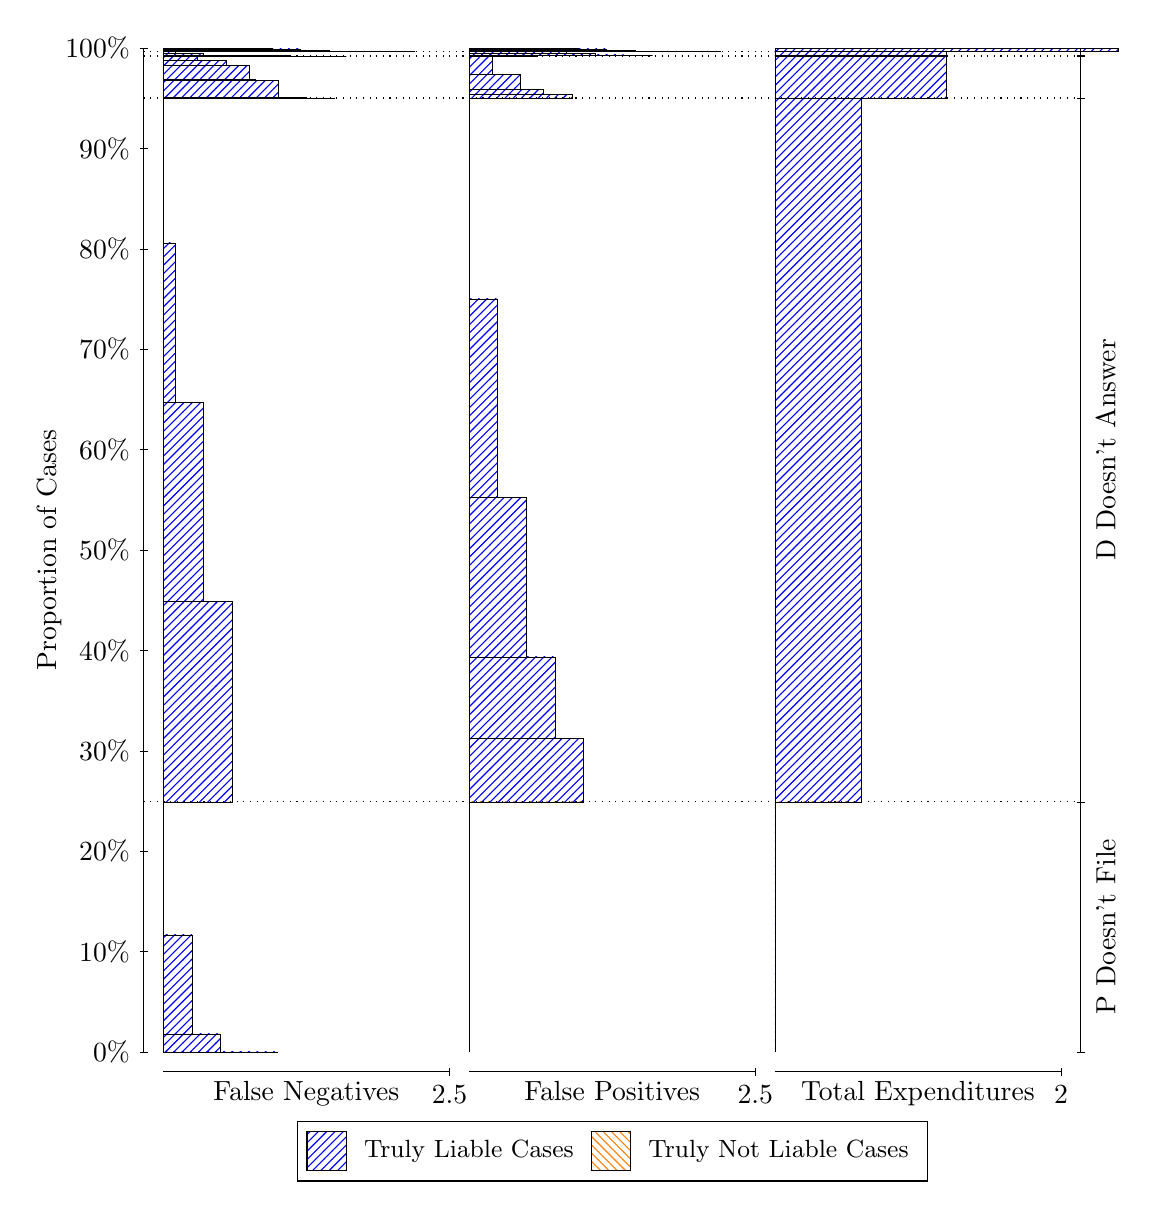
\begin{tikzpicture}
\draw[black, very thin] (1.5,1.75) -- (1.5,14.5);
\node[rotate=90, text=black, anchor=center] at (0.3, 8.125) {Proportion of Cases};
\draw[black, very thin] (1.45,1.75) -- (1.55,1.75);
\node[text=black, anchor=east] at (1.45, 1.75) {0\%};
\draw[black, very thin] (1.45,3.025) -- (1.55,3.025);
\node[text=black, anchor=east] at (1.45, 3.025) {10\%};
\draw[black, very thin] (1.45,4.3) -- (1.55,4.3);
\node[text=black, anchor=east] at (1.45, 4.3) {20\%};
\draw[black, very thin] (1.45,5.575) -- (1.55,5.575);
\node[text=black, anchor=east] at (1.45, 5.575) {30\%};
\draw[black, very thin] (1.45,6.85) -- (1.55,6.85);
\node[text=black, anchor=east] at (1.45, 6.85) {40\%};
\draw[black, very thin] (1.45,8.125) -- (1.55,8.125);
\node[text=black, anchor=east] at (1.45, 8.125) {50\%};
\draw[black, very thin] (1.45,9.4) -- (1.55,9.4);
\node[text=black, anchor=east] at (1.45, 9.4) {60\%};
\draw[black, very thin] (1.45,10.675) -- (1.55,10.675);
\node[text=black, anchor=east] at (1.45, 10.675) {70\%};
\draw[black, very thin] (1.45,11.95) -- (1.55,11.95);
\node[text=black, anchor=east] at (1.45, 11.95) {80\%};
\draw[black, very thin] (1.45,13.225) -- (1.55,13.225);
\node[text=black, anchor=east] at (1.45, 13.225) {90\%};
\draw[black, very thin] (1.45,14.5) -- (1.55,14.5);
\node[text=black, anchor=east] at (1.45, 14.5) {100\%};

\draw[black, very thin] (13.4,1.75) -- (13.4,14.5);
\draw[black, very thin] (13.35,1.75) -- (13.45,1.75);
\node[anchor=west] at (13.35, 1.75) {};
\draw[black, very thin] (13.35,4.9274) -- (13.45,4.9274);
\node[anchor=west] at (13.35, 4.9274) {};
\draw[black, very thin] (13.35,13.865) -- (13.45,13.865);
\node[anchor=west] at (13.35, 13.865) {};
\draw[black, very thin] (13.35,14.393) -- (13.45,14.393);
\node[anchor=west] at (13.35, 14.393) {};
\draw[black, very thin] (13.35,14.41) -- (13.45,14.41);
\node[anchor=west] at (13.35, 14.41) {};
\draw[black, very thin] (13.35,14.457) -- (13.45,14.457);
\node[anchor=west] at (13.35, 14.457) {};
\draw[black, very thin] (13.35,14.5) -- (13.45,14.5);
\node[anchor=west] at (13.35, 14.5) {};

\draw[black, very thin, pattern color=blue, pattern=north east lines] (1.75,1.75) rectangle (3.2033,1.75);
\draw[black, very thin, pattern color=blue, pattern=north east lines] (1.75,1.75) rectangle (2.84,1.7519);
\draw[black, very thin, pattern color=blue, pattern=north east lines] (1.75,1.7519) rectangle (2.4767,1.98);
\draw[black, very thin, pattern color=blue, pattern=north east lines] (1.75,1.98) rectangle (2.1133,3.2367);
\draw[black, very thin, pattern color=orange, pattern=north west lines] (1.75,3.2367) rectangle (1.75,3.2367);
\draw[black, very thin, pattern color=blue, pattern=north east lines] (1.75,3.2367) rectangle (1.75,4.9274);
\draw[black, very thin, pattern color=blue, pattern=north east lines] (1.75,4.9274) rectangle (2.622,7.477);
\draw[black, very thin, pattern color=blue, pattern=north east lines] (1.75,7.477) rectangle (2.2587,9.9966);
\draw[black, very thin, pattern color=blue, pattern=north east lines] (1.75,9.9966) rectangle (1.8953,12.024);
\draw[black, very thin, pattern color=orange, pattern=north west lines] (1.75,12.024) rectangle (1.75,12.024);
\draw[black, very thin, pattern color=blue, pattern=north east lines] (1.75,12.024) rectangle (1.75,13.865);
\draw[black, very thin, pattern color=blue, pattern=north east lines] (1.75,13.865) rectangle (3.93,13.865);
\draw[black, very thin, pattern color=blue, pattern=north east lines] (1.75,13.865) rectangle (3.6393,13.865);
\draw[black, very thin, pattern color=blue, pattern=north east lines] (1.75,13.865) rectangle (3.5667,13.869);
\draw[black, very thin, pattern color=blue, pattern=north east lines] (1.75,13.869) rectangle (3.276,13.869);
\draw[black, very thin, pattern color=blue, pattern=north east lines] (1.75,13.869) rectangle (3.2033,14.093);
\draw[black, very thin, pattern color=blue, pattern=north east lines] (1.75,14.093) rectangle (2.9127,14.097);
\draw[black, very thin, pattern color=blue, pattern=north east lines] (1.75,14.097) rectangle (2.84,14.282);
\draw[black, very thin, pattern color=blue, pattern=north east lines] (1.75,14.282) rectangle (2.5493,14.341);
\draw[black, very thin, pattern color=blue, pattern=north east lines] (1.75,14.341) rectangle (2.4767,14.343);
\draw[black, very thin, pattern color=blue, pattern=north east lines] (1.75,14.343) rectangle (2.186,14.393);
\draw[black, very thin, pattern color=orange, pattern=north west lines] (1.75,14.393) rectangle (1.75,14.393);
\draw[black, very thin, pattern color=blue, pattern=north east lines] (1.75,14.393) rectangle (4.0753,14.393);
\draw[black, very thin, pattern color=blue, pattern=north east lines] (1.75,14.393) rectangle (3.712,14.393);
\draw[black, very thin, pattern color=blue, pattern=north east lines] (1.75,14.393) rectangle (3.3487,14.402);
\draw[black, very thin, pattern color=blue, pattern=north east lines] (1.75,14.402) rectangle (2.9853,14.41);
\draw[black, very thin, pattern color=blue, pattern=north east lines] (1.75,14.41) rectangle (2.622,14.41);
\draw[black, very thin, pattern color=orange, pattern=north west lines] (1.75,14.41) rectangle (1.75,14.41);
\draw[black, very thin, pattern color=blue, pattern=north east lines] (1.75,14.41) rectangle (2.622,14.411);
\draw[black, very thin, pattern color=blue, pattern=north east lines] (1.75,14.411) rectangle (2.2587,14.433);
\draw[black, very thin, pattern color=blue, pattern=north east lines] (1.75,14.433) rectangle (1.8953,14.456);
\draw[black, very thin, pattern color=orange, pattern=north west lines] (1.75,14.456) rectangle (1.75,14.456);
\draw[black, very thin, pattern color=blue, pattern=north east lines] (1.75,14.456) rectangle (1.75,14.457);
\draw[black, very thin, pattern color=blue, pattern=north east lines] (1.75,14.457) rectangle (4.9473,14.457);
\draw[black, very thin, pattern color=blue, pattern=north east lines] (1.75,14.457) rectangle (4.584,14.457);
\draw[black, very thin, pattern color=blue, pattern=north east lines] (1.75,14.457) rectangle (4.2207,14.458);
\draw[black, very thin, pattern color=blue, pattern=north east lines] (1.75,14.458) rectangle (3.8573,14.468);
\draw[black, very thin, pattern color=blue, pattern=north east lines] (1.75,14.468) rectangle (3.494,14.489);
\draw[black, very thin, pattern color=blue, pattern=north east lines] (1.75,14.489) rectangle (3.1307,14.499);
\draw[black, very thin, pattern color=blue, pattern=north east lines] (1.75,14.499) rectangle (2.7673,14.5);
\draw[black, very thin, pattern color=blue, pattern=north east lines] (1.75,14.5) rectangle (2.404,14.5);
\draw[black, very thin, pattern color=blue, pattern=north east lines] (1.75,14.5) rectangle (2.0407,14.5);
\draw[black, very thin, pattern color=orange, pattern=north west lines] (1.75,14.5) rectangle (1.75,14.5);
\draw[black, very thin, pattern color=orange, pattern=north west lines] (5.6333,1.75) rectangle (5.6333,1.75);
\draw[black, very thin, pattern color=blue, pattern=north east lines] (5.6333,1.75) rectangle (5.6333,4.9274);
\draw[black, very thin, pattern color=orange, pattern=north west lines] (5.6333,4.9274) rectangle (7.0867,4.9274);
\draw[black, very thin, pattern color=blue, pattern=north east lines] (5.6333,4.9274) rectangle (7.0867,5.7343);
\draw[black, very thin, pattern color=blue, pattern=north east lines] (5.6333,5.7343) rectangle (6.7233,6.7684);
\draw[black, very thin, pattern color=blue, pattern=north east lines] (5.6333,6.7684) rectangle (6.36,8.7959);
\draw[black, very thin, pattern color=blue, pattern=north east lines] (5.6333,8.7959) rectangle (5.9967,11.315);
\draw[black, very thin, pattern color=blue, pattern=north east lines] (5.6333,11.315) rectangle (5.6333,13.865);
\draw[black, very thin, pattern color=orange, pattern=north west lines] (5.6333,13.865) rectangle (6.9413,13.865);
\draw[black, very thin, pattern color=blue, pattern=north east lines] (5.6333,13.865) rectangle (6.9413,13.915);
\draw[black, very thin, pattern color=orange, pattern=north west lines] (5.6333,13.915) rectangle (6.6507,13.915);
\draw[black, very thin, pattern color=blue, pattern=north east lines] (5.6333,13.915) rectangle (6.6507,13.917);
\draw[black, very thin, pattern color=blue, pattern=north east lines] (5.6333,13.917) rectangle (6.578,13.976);
\draw[black, very thin, pattern color=blue, pattern=north east lines] (5.6333,13.976) rectangle (6.2873,14.161);
\draw[black, very thin, pattern color=blue, pattern=north east lines] (5.6333,14.161) rectangle (6.2147,14.165);
\draw[black, very thin, pattern color=blue, pattern=north east lines] (5.6333,14.165) rectangle (5.924,14.389);
\draw[black, very thin, pattern color=blue, pattern=north east lines] (5.6333,14.389) rectangle (5.8513,14.389);
\draw[black, very thin, pattern color=blue, pattern=north east lines] (5.6333,14.389) rectangle (5.6333,14.393);
\draw[black, very thin, pattern color=orange, pattern=north west lines] (5.6333,14.393) rectangle (6.5053,14.393);
\draw[black, very thin, pattern color=blue, pattern=north east lines] (5.6333,14.393) rectangle (6.5053,14.393);
\draw[black, very thin, pattern color=blue, pattern=north east lines] (5.6333,14.393) rectangle (6.142,14.402);
\draw[black, very thin, pattern color=blue, pattern=north east lines] (5.6333,14.402) rectangle (5.7787,14.41);
\draw[black, very thin, pattern color=blue, pattern=north east lines] (5.6333,14.41) rectangle (5.6333,14.41);
\draw[black, very thin, pattern color=orange, pattern=north west lines] (5.6333,14.41) rectangle (7.9587,14.41);
\draw[black, very thin, pattern color=blue, pattern=north east lines] (5.6333,14.41) rectangle (7.9587,14.41);
\draw[black, very thin, pattern color=blue, pattern=north east lines] (5.6333,14.41) rectangle (7.5953,14.412);
\draw[black, very thin, pattern color=blue, pattern=north east lines] (5.6333,14.412) rectangle (7.232,14.434);
\draw[black, very thin, pattern color=blue, pattern=north east lines] (5.6333,14.434) rectangle (6.8687,14.457);
\draw[black, very thin, pattern color=blue, pattern=north east lines] (5.6333,14.457) rectangle (6.5053,14.457);
\draw[black, very thin, pattern color=orange, pattern=north west lines] (5.6333,14.457) rectangle (8.8307,14.457);
\draw[black, very thin, pattern color=blue, pattern=north east lines] (5.6333,14.457) rectangle (8.8307,14.457);
\draw[black, very thin, pattern color=blue, pattern=north east lines] (5.6333,14.457) rectangle (8.4673,14.457);
\draw[black, very thin, pattern color=orange, pattern=north west lines] (5.6333,14.457) rectangle (8.4673,14.457);
\draw[black, very thin, pattern color=blue, pattern=north east lines] (5.6333,14.457) rectangle (8.4673,14.457);
\draw[black, very thin, pattern color=blue, pattern=north east lines] (5.6333,14.457) rectangle (8.104,14.458);
\draw[black, very thin, pattern color=orange, pattern=north west lines] (5.6333,14.458) rectangle (8.104,14.458);
\draw[black, very thin, pattern color=blue, pattern=north east lines] (5.6333,14.458) rectangle (8.104,14.458);
\draw[black, very thin, pattern color=blue, pattern=north east lines] (5.6333,14.458) rectangle (7.7407,14.458);
\draw[black, very thin, pattern color=orange, pattern=north west lines] (5.6333,14.458) rectangle (7.7407,14.458);
\draw[black, very thin, pattern color=blue, pattern=north east lines] (5.6333,14.458) rectangle (7.7407,14.468);
\draw[black, very thin, pattern color=blue, pattern=north east lines] (5.6333,14.468) rectangle (7.3773,14.468);
\draw[black, very thin, pattern color=orange, pattern=north west lines] (5.6333,14.468) rectangle (7.3773,14.468);
\draw[black, very thin, pattern color=blue, pattern=north east lines] (5.6333,14.468) rectangle (7.3773,14.489);
\draw[black, very thin, pattern color=blue, pattern=north east lines] (5.6333,14.489) rectangle (7.014,14.499);
\draw[black, very thin, pattern color=blue, pattern=north east lines] (5.6333,14.499) rectangle (6.6507,14.5);
\draw[black, very thin, pattern color=blue, pattern=north east lines] (5.6333,14.5) rectangle (6.2873,14.5);
\draw[black, very thin, pattern color=blue, pattern=north east lines] (5.6333,14.5) rectangle (5.924,14.5);
\draw[black, very thin, pattern color=orange, pattern=north west lines] (9.5167,1.75) rectangle (9.5167,1.75);
\draw[black, very thin, pattern color=blue, pattern=north east lines] (9.5167,1.75) rectangle (9.5167,4.9274);
\draw[black, very thin, pattern color=orange, pattern=north west lines] (9.5167,4.9274) rectangle (10.607,4.9274);
\draw[black, very thin, pattern color=blue, pattern=north east lines] (9.5167,4.9274) rectangle (10.607,13.865);
\draw[black, very thin, pattern color=orange, pattern=north west lines] (9.5167,13.865) rectangle (11.697,13.865);
\draw[black, very thin, pattern color=blue, pattern=north east lines] (9.5167,13.865) rectangle (11.697,14.393);
\draw[black, very thin, pattern color=orange, pattern=north west lines] (9.5167,14.393) rectangle (11.697,14.393);
\draw[black, very thin, pattern color=blue, pattern=north east lines] (9.5167,14.393) rectangle (11.697,14.41);
\draw[black, very thin, pattern color=orange, pattern=north west lines] (9.5167,14.41) rectangle (11.697,14.41);
\draw[black, very thin, pattern color=blue, pattern=north east lines] (9.5167,14.41) rectangle (11.697,14.457);
\draw[black, very thin, pattern color=orange, pattern=north west lines] (9.5167,14.457) rectangle (13.877,14.457);
\draw[black, very thin, pattern color=blue, pattern=north east lines] (9.5167,14.457) rectangle (13.877,14.458);
\draw[black, very thin, pattern color=orange, pattern=north west lines] (9.5167,14.458) rectangle (13.877,14.458);
\draw[black, very thin, pattern color=blue, pattern=north east lines] (9.5167,14.458) rectangle (13.877,14.5);
\draw[black, dotted] (1.5,4.9274) -- (13.4,4.9274);
\draw[black, dotted] (1.5,13.865) -- (13.4,13.865);
\draw[black, dotted] (1.5,14.393) -- (13.4,14.393);
\draw[black, dotted] (1.5,14.41) -- (13.4,14.41);
\draw[black, dotted] (1.5,14.457) -- (13.4,14.457);
\draw[black, very thin] (1.75,1.5) -- (5.3833,1.5);
\node[text=black, anchor=north] at (3.5667, 1.5) {False Negatives};
\draw[black, very thin] (5.3833,1.45) -- (5.3833,1.55);
\node[text=black, anchor=north] at (5.3833, 1.45) {2.5};

\draw[black, very thin] (5.6333,1.5) -- (9.2667,1.5);
\node[text=black, anchor=north] at (7.45, 1.5) {False Positives};
\draw[black, very thin] (9.2667,1.45) -- (9.2667,1.55);
\node[text=black, anchor=north] at (9.2667, 1.45) {2.5};

\draw[black, very thin] (9.5167,1.5) -- (13.15,1.5);
\node[text=black, anchor=north] at (11.333, 1.5) {Total Expenditures};
\draw[black, very thin] (13.15,1.45) -- (13.15,1.55);
\node[text=black, anchor=north] at (13.15, 1.45) {2};

\node[text=black, centered, rotate=90] at (13.72, 3.3387) {P Doesn't File};
\node[text=black, centered, rotate=90] at (13.72, 9.3963) {D Doesn't Answer};





\draw (7.449999999999999,1.5) node[draw=none] (baseCoordinate) {};
\begin{scope}[align=center]
        \matrix[scale=0.5, draw=black, below=0.5cm of baseCoordinate, nodes={draw}, column sep=0.1cm]{
            \node[rectangle, draw, minimum width=0.5cm, minimum height=0.5cm, pattern color=blue, pattern=north east lines] {}; &
            \node[draw=none, font=\small, text=black] (B) {Truly Liable Cases}; &
            \node[rectangle, draw, minimum width=0.5cm, minimum height=0.5cm, pattern color=orange, pattern=north west lines] {}; &
            \node[draw=none, font=\small, text=black] (B) {Truly Not Liable Cases}; \\
            };
\end{scope}

\end{tikzpicture}
\end{document}